\documentclass[12pt]{article}
\usepackage{pagestyle}

\begin{document}
\thispagestyle{empty}

{\scshape ML } \hfill {\scshape \large application guide} \hfill {\scshape 20.02.2024}

\smallskip
\hrule
\bigskip

\tableofcontents

\section{Gradients}
For this type of question you more or less just have to memorize the rules on the sheet.

\section{Entropy}

You are given the formulas but it helps to understand the intition behind them. 

\smallskip
\subsection{Entropy of a random variable}
As a simple reminder, the code length (number of bits required to represent a certain probability) of a random variable $X$ under a probability distribution $p(x)$ is given by
\[
    L(x) = -\log_2 p(x)
\]
So the expected code length over the entire distribution is
\[
    \EX{L(x)} = \sum_{x\in X}p(x)L(x) = -\sum_{x\in X}p(x)\log_2 p(x) = H(X)
\]
Which is also called the entropy of the random variable $X$ and is denoted by $H(X)$. This is technically the same thing as the entropy of a probability distribution $p(x)$, which is commonly written as $H(p(x))$ or just $H(p)$. A key thing to remember, as the probability of an event decreases, the code length increases (since we need more bits to represent this number), hence the entropy increases.
\smallskip
\subsubsection*{application}
Applying this is generally simple, if you are given some variables $\{x_1, x_2, \ldots, x_n\}$. Then to compute $H(p)$ you just have to compute
\[
    H(p) = -\sum_{i=1}^{n}p(x_i)\log_2 p(x_i)
\]
\subsection{Cross entropy}
Cross entropy is a measure of the distance between two probability distribitons $p$ and $q$. The formula again is just a simple extension of the entropy formula.
\[
    H(p, q) = \EX_p{L(q)} = \sum_{x\in X}p(x)L(q) = -\sum_{x\in X}p(x)\log_2 q(x)
\] 
Its a measure of the distance by the simple fact that if $p$ and $q$ are the same, then the cross entropy is the same as the entropy of $p$. As $q$ diverges from $p$, the cross entropy increases, hence the `distance' increases.
\subsubsection*{application}
Again here you will usually have the same pattern of being given some set of variables, usually in a table, and you just compute the cross entropy applying the formula.

\subsection{Conditional entropy}
The conditional entropy is just the entropy of a random variable given another random variable. The formula is
\[
    H(X\mid Y) = \EX{L(X\mid Y)} = \sum_{y\in Y}p(y)L(X\mid Y) = -\sum_{y\in Y}p(y)\sum_{x\in X}p(x\mid y)\log_2 p(x\mid y)  
\]

\section{Evidence Lower Bound}
Prof here says key thing is to understand the derivation. Realistically the main thing you need to understand is that basically all of the manipulations done from line to line are just applications of two basic rules. The most important to understand is bayes in this context
\[
    p(x\mid z) = \frac{p(z\mid x)p(x)}{p(z)} = \frac{p(x, z)}{p(z)}\implies p(z) = \frac{p(x, z)}{p(x\mid z)}
\]
\textbf{Of note} is that prof I think is a bit weird with notation, technically you write $p_\theta(x, z)$ and $q_\phi(x, z)$ but it seems here he just does $p(x, z\mid \theta) = p_\theta(x, z)$ and $q(x, z) = q_\phi(x, z)$, probably. Bit of a random nitpick though.  

In regards to log rules you more or less just have to remember the divison rule
\[
    \ln \frac{a}{b} = \ln a - \ln b    
\]
\subsection{Full derivation}

For brevity I will just exclude the conditional parameters $\theta$ and $\phi$ since they are usually implied anyways. 


\begin{align}
    L(q, \theta) + KL(q, p) &= \EX_q\ln \frac{p(x, z)}{q(z\mid x)} - \EX_q \ln \frac{p(z\mid x)}{q(z\mid x)} \\
    &= \EX_q \ln p(x, z) - \EX_q \ln q(z\mid x) - \EX_q \ln (z\mid x) + \EX_q(z\mid x) \quad (\text{log div.}) \\
    &= \EX_q \ln p(x, z) - \EX_q \ln p(z\mid x)\quad (\text{simplification}) \\
    &= \EX_q \ln \frac{p(x, z)}{p(z\mid x)} \quad (\text{log division})\\
    &= \EX_q \ln \frac{p(z\mid x)p(x)}{p(z\mid x)} \quad (\text{bayes}) \\
    &= \EX_q \ln p(x) \quad (\text{simplification})\\
\end{align}

You should be able to now follow the derivations, put in plain english we can explain the steps as 
\begin{enumerate}[leftmargin=*, noitemsep]
    \item We start with the definition of the ELBO and the KL divergence.
    \item We apply the log rule for division and then expand both logarithms 
    \item We cancel out the same terms 
    \item We apply log rule for divison just in reverse so subtraction $\rightarrow$ divison
    \item We just rewrite the joint distribution into the equivalent form, so just Bayes again
    \item We divide out common terms 
\end{enumerate}

So you can kinda see, its literally just applying the formula for $p(x\mid z)$ (and flipped) and then applying the log rule for division. You just have to remember the definition of $L$, $KL$ formula is provided on the sheet.
\subsection{Additional notes}
The general objective with the ELBO is to maximize it, or equivalently (and more commonly) minimize it. The loss function is usually written as the negative ELBO ($L$ function previously)
\[
    -L(q, \theta) = \underbrace{KL(q(z\mid x), p(z))}_{\text{regularization term}} - \underbrace{\EX_q\ln p(x\mid z)}_{\text{reconstruction error}}
\]
All this function is is just the ELBO term rewritten into two terms that express its meaning more clearly.
\begin{itemize}[leftmargin=*, noitemsep]
    \item $p(z)$ is the assumed prior distribution, \textbf{on the exam they expect $N(0, 1)$ (standard normal)}
    \item The regularization term \textbf{prevents overfitting} by ensuring the learned distribution $q(z\mid x)$ does not diverge too much from the prior $p(z)$.
    \item The reconstruction error \textbf{improves the model} by ensuring that the learned distribution $q(z\mid x)$ can accurately reconstruct the input $x$.
\end{itemize}

\section{Backpropagation and Matrix Backpropagation}

\subsection{Breaking into modules}

A common starting point is breaking the function into modules. That is, we create a composition of basic functions that we can then in turn differentiate applying the chain rule.

\smallskip
The \textbf{multivariate chain rule} is the most important thing to remember here, especially then visual intuition in terms of the computation graphs. First we can look at a simple composite 
\[
    f(x) = g(h(x))\implies \frac{\partial f}{\partial x} = \frac{\partial g}{\partial h}\frac{\partial h}{\partial x}     
\]
In this instance the computation graph looks as follows
\begin{figure}[!h]
    \centering
    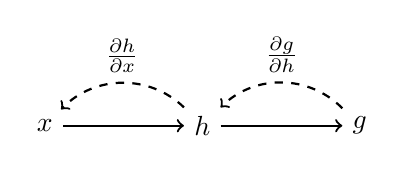
\begin{tikzpicture}
        [
            ->, 
            auto, 
            thick, 
            node/.style={circle, draw, font=\sffamily\Large\bfseries}
        ]
        \node (x) at (0, 0) {$x$};
        \node (h) at (2, 0) {$h$};
        \node (g) at (4, 0) {$g$};
        \path[every node=/.style={font=\sffamily\small}]
        (x) edge node [right] {} (h)
        (h) edge node [right] {} (g);

        \draw[dashed, ->] (g) to [bend right=45] node [above] {$\frac{\partial g}{\partial h}$} (h);
        \draw[dashed, ->] (h) to [bend right=45] node [above] {$\frac{\partial h}{\partial x}$} (x);
    \end{tikzpicture}

\end{figure}

A question only big math nerds have at this point is, `what if you don't have a simple composition?', that is, what if you have something like 
\[
    f(x) = f(c(a(x)b(x)))   
\]
Because I like doing things in a bad order lets just write out the full derivation and kinda work backwards, so applying the chain rule we get 
\begin{align*}
    \frac{\partial f}{\partial x} &= \frac{\partial f}{\partial c}\left( \frac{\partial c}{\partial a} \frac{\partial a}{\partial x} + \frac{\partial c}{\partial b}\frac{\partial b}{\partial x} \right) \\ 
    &= \frac{\partial f}{\partial c}\frac{\partial c}{\partial a}\frac{\partial a}{\partial x} + \frac{\partial f}{\partial c}\frac{\partial c}{\partial b}\frac{\partial b}{\partial x}
\end{align*}

Now initially this looks a bit weird but lets again draw the computation graph \\
\begin{figure}[!h]
    \centering
    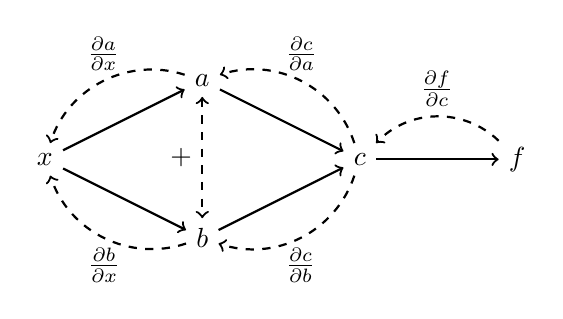
\begin{tikzpicture}
        [
            ->, 
            auto, 
            thick, 
            node/.style={circle, draw, font=\sffamily\Large\bfseries}
        ]
        \node (x) at (0, 0) {$x$};
        \node (a) at (2, 1) {$a$};
        \node (b) at (2, -1) {$b$};
        \node (c) at (4, 0) {$c$};
        \node (f) at (6, 0) {$f$};
        \path[every node=/.style={font=\sffamily\small}]
        (x) edge node [right] {} (a)
        (x) edge node [right] {} (b)
        (a) edge node [right] {} (c)
        (b) edge node [right] {} (c)
        (c) edge node [right] {} (f);

        \draw[dashed, ->] (f) to [bend right=45] node [above] {$\frac{\partial f}{\partial c}$} (c);
        \draw[dashed, ->] (c) to [bend right=45] node [above] {$\frac{\partial c}{\partial a}$} (a);
        \draw[dashed, ->] (c) to [bend left=45] node [below] {$\frac{\partial c}{\partial b}$} (b);
        \draw[dashed, ->] (a) to [bend right=45] node [above] {$\frac{\partial a}{\partial x}$} (x);
        \draw[dashed, ->] (b) to [bend left=45] node [below] {$\frac{\partial b}{\partial x}$} (x);
        \draw[dashed, <->] (a) to node [left] {$+$} (b);

    \end{tikzpicture}
\end{figure}

So again you can see that its the same idea as the linear chain rule, but we just sum over all the paths. 

\section{Decision Trees}

These questions usually follow a roughly similar format, you are generally given a table containing some set of features, lets call them $\{x_1, x_2, \ldots, x_n\}$ and usually one target which we can call $y$. 
\smallskip 

The first thing you always do is calculate the entropy of the target variable $y$. This is just the entropy of the distribution of $y$ over the entire dataset. So you tally the number of unique instances of $y$ and then calculate the entropy using the formula
\[
    H(y) = -\sum_{i=1}^{n}p(y_i)\log_2 p(y_i)
\]
The tables generally have one axis as the target labels, so the labels of $y$, then the other axis as the features. So the actual values the features can take on, such as `Sunny', in the case of $x_1 = \text{Weather}$ etc. 
\smallskip

\textbf{The cells} of this table are then simply the counts of the number of instances where the feature $x_i$ takes on a certain value and the target $y$ takes on a certain value. For example the cell (sunny, yes) for the split of a weather feature would be the number of instances where the weather feature takes ont he sunny value and the corresponding target take on the yes value. 
\smallskip

\textbf{The information gain} for each feature is then calculated using the following formula. 
\[
    I(y, x_i) = H(y) - H(y\mid x_i) = H(y) - \sum_{x_j\in x_i}p(x_{j})H(y\mid x_{ij})
\]
How you use this generally goes as follows 
\begin{enumerate}[leftmargin=*, noitemsep]
    \item Compute $H(y)$, you will probably have already done this 
    \item For each feature $x_i$ compute $H(y\mid x_i)$ and $p(x_{j})$ for each value of $x_i$
\end{enumerate}

Best to demonstrate this with an example, we have the following table 
\begin{figure}[!h]
    \centering
    \includegraphics[width=0.4\textwidth]{assets/dt1.png}
\end{figure}
\begin{enumerate}
    \item First we compute $H(\text{Bites})$
    \begin{align*}
        H(\text{Bites}) &= \sum_{x\in \text{Bites}}p(x)L(x) \\
                        &= p(\text{Yes})L(\text{Yes}) + p(\text{No})L(\text{No}) \\
                        &= -\frac{5}{8}\log_2\frac{5}{8} - \frac{3}{8}\log_2\frac{3}{8} \\
                        &\approx 0.9544
    \end{align*}
    \item Then we make the tables for each feature 
    \begin{figure}[!h]
        \centering
        \includegraphics[width=0.5\textwidth]{assets/dt2.png}
    \end{figure}\\
    If you are confused just remember that the cells are just tallies/counts of where a certain value of a feature corresponds to a certain value of the target. For example in the big table we can see Heavy having the target value Yes occurs 2 times with Bites also having a value Yes.
    \item Then we compute the information gain for each feature, remember the formula has two parts, the marginal probabilities of the features, and the conditional entropy of the target given the feature. Using the \textit{Growling} table as an example 
    \begin{itemize}
        \item The marginal probabilities are 
        \[
            p(\text{Growling} = \text{Yes}) = \frac{3}{8} + \frac{1}{8} = \frac{4}{8} \quad
            p(\text{Growling} = \text{No}) = \frac{2}{8} + \frac{2}{8} = \frac{4}{8}
        \]
        \item To then compute the conditional entropy we use the formula
        \begin{align*}
            H(\text{Bites}\mid \text{Growling}) &= \sum_{g\in \text{Growling}}p(g)H(\text{Bites}\mid g) \\
            &= \frac{4}{8}H(\text{Bites}\mid \text{Growling} = \text{Yes}) + \frac{4}{8}H(\text{Bites}\mid \text{Growling} = \text{No}) \\
            &= \frac{4}{8}\left(-\frac{3}{4}\log_2\frac{3}{4} - \frac{1}{4}\log_2\frac{1}{4}\right) + \frac{4}{8}\left(-\frac{1}{2}\log_2\frac{1}{2} - \frac{1}{2}\log_2\frac{1}{2}\right) \\
            &\approx 0.9056
        \end{align*}
    \end{itemize}
    \item Once we have computed the largest information gain we again split now on a feature, in our case \textit{Growling}. We then repeat the process for each of the new tables. These new tables work as follows 
    \begin{itemize}
        \item Ignore the column of the feature we split on, if we split on \textit{Growling} then ignore the \textit{Growling} column.
        \item Each branch corresponds to a value of the feature, e.g. Yes, and for each branch the table we consider contains only those rows where the feature (e.g. Growling) has the value of the branch (e.g. Yes).
    \end{itemize}
    \begin{figure}[!h]
        \centering
        \includegraphics[width=0.8\textwidth]{assets/dt3.png}
    \end{figure} 
    Here you can see the \textit{Growling} column being ignored (greyed out) and the tables being split by the feature, so where \textit{Growling} is Yes and No.
    \item We then repeat the process for each of the new tables, computing the entropy of the target, the marginal probabilities of the features, and the conditional entropy of the target given the feature.
\end{enumerate}

\section{Naive Bayes}

I'm gonna basically paraphrase wikipedia here because I like how they describe it. So Naive Bayes is a \textit{conditional probability model} that assigns the probability of a class $C_k$ for each $K$ outcome given some instance to be classified $\mathbf x = \{x_1, x_2, \dots, x_n\}$ with $n$ features. Using Bayes theorem we can write the probability of a class given the features as
\[
    P(C_k\mid \mathbf x) = \frac{P(\mathbf x\mid C_k)P(C_k)}{P(\mathbf x)}    
\]
Now the issue is that if the number of features is large then the problem in simple terms becomes intractable, that is it becomes too computationally expensive. So the `naive' part of Naive Bayes is that we assume that the features are conditionally independent given the class. So we make the following assumption 
\[
    P(\mathbf x\mid C_k) = P(x_1\mid C_k)P(x_2\mid C_k)\dots P(x_n\mid C_k)    
\]
Thus we can express the joint model, so the model expressing the probability of features for a class, as 
\[
    P(C_k\mid \mathbf x) = \frac{1}{Z}P(C_k)\prod_{i=1}^{n}P(x_i\mid C_k)
\]
$Z$ in this case is just $p(\mathbf x)$, the probability of the features, and is constant if the features are known, we generall exclude this and just say 
\[
    P(C_k\mid \mathbf x) \propto P(C_k)\prod_{i=1}^{n}P(x_i\mid C_k)    
\]

\subsection{Issues and smoothing}

Smoothing is a technique used to handle the issue of zero probabilities. That is, if a feature value does not occur in the training set for a class then the probability of that feature given the class is zero. This is an issue because then the entire probability of the class given the features is zero. Formally 
\[
    p(x_m\mid C_k) = 0 \implies \prod_{i=1}^{n}P(x_i\mid C_k) = 0 \quad 1\leq m\leq n
\]

There are two solutions to this first we have the normal \textbf{smoothing} which works as follows
\[
    p(x_i\mid C_k) = \frac{N_{ic} + \alpha}{N_c + \alpha n}
\]
Where $N_{ic}$ is the number of times feature $i$ appears in class $c$, $N_c$ is the number of times class $c$ appears in the training set, $\alpha$ is the smoothing parameter, and $n$ is the number of features. The other solution is \textbf{Laplace smoothing} which is just the case where $\alpha = 1$.
\[
    p(x_i\mid C_k) = \frac{N_{ic} + 1}{N_c + n}    
\]
What this means in practice is for example in the case of Laplace smoothing, if a particular feature, say $x_i$ for $n = 2$ does not appear in the training set for a class $C_k$ then the probability of that feature given the class is
\[
    p(x_i\mid C_k) = \frac{0 + 1}{0 + 2} = \frac{1}{2}    
\]

\subsection{application} 
Lets take the following table
\begin{figure}[!h]
    \centering
    \includegraphics[width=0.25\textwidth]{assets/hb1.png}
    \caption{Table of features and class labels with smoothing added}
\end{figure}

\subsubsection*{Smoothing}

Sometimes questions might ask what a smoothed naive bayes would compute. In this case we can use simple Laplace smoothing, which just means ensuring that each feature is seen at least once in each class. So pill is both truthy and falsey in the spam class, and meeting is both truthy and falsey in the ham class. This is just to ensure that the probability of a feature given a class is never zero.

\subsubsection*{Creating the model}

So, first thing to generally do here is compute the marginal for the classes 
\[
    p(\text{Spam}) = \frac{4}{8} \quad p(\text{Ham}) = \frac{4}{8}    
\]
With this in mind, and remembering the conditional independence rule, so just splitting the conditional probabilities into its components, we can solve Naive Bayes questions as follows. 

\smallskip
Usually you are going to be prompted with an instance which has certain features, lets say an email $e$ with the features $\mathbf x = (\text{`pill'} = T, \text{`meeting'} = F)$. To then solve any conditional we simply apply the formula, that is 
\begin{align*}
    p(\text{Class} \mid \mathbf x) &\propto p(\text{Class})\prod_{i=1}^{n}p(x_i\mid \text{Class}) \\
    &= p(\text{Class})p(\text{`pill'} = T \mid \text{Class})p(\text{`meeting'} = T \mid \text{Class}) 
\end{align*}
There are two cases now where we apply this logic. 
\subsubsection*{Comparison}

For comparison questions that do not mention probabilities explicitly we can rely on the proportionality of the conditional probabilities to determine the class. Specifically, for some set of classes $\mathbf C = \{C_1, C_2, \ldots, C_n\}$ to determine the chosen clase for a given instance $\mathbf x$ we compute all 
\[
    p(C_k\mid \mathbf x) \propto p(C_k)\prod_{i=1}^{n}p(x_i\mid C_k)    
\]
And then choose the class with the highest proportional probability.

\subsubsection*{Probability}

If the question explicitly asks for the probabilites of two different classes then we must divide by the marginal to normalize the probabilities (make them sum to 1). So again given some feature $\mathbf x$ we compute the probabilities as
\[
    p(C_k\mid \mathbf x) = \frac{p(C_k)\prod_{i=1}^{n}p(x_i\mid C_k)}{p(\mathbf x)}    
\]

\subsection{Summary: I'm still confused}
To summarize, generally you are given a table, usually with some target classes, we can call them $\{C_1, C_2, \ldots, C_n\}$ and some features $\{x_1, x_2, \ldots, x_n\}$. These features can adopt some set of values $\{T, F\}$, or \{Sunny, Rainy, Overcast\} etc. 
\begin{enumerate}[leftmargin=*, noitemsep]
    \item The first thing you do is compute the marginal probabilities of the classes, so $p(C_k)$.
    \item Then you see the instance you are given, you then compute the conditional probabilities of the features given the class, so $p(x_i\mid C_k)$.
    \item If you are asked to compare the probabilities of two classes you just compute the proportional probabilities (numerator) and then choose the class with the highest probability, otherwise you normalize the probabilities by dividing by the marginal. 
\end{enumerate}

\section{Support Vector Machine}

\section{Markov Model}

These questions usually start off with some instance, say an email, to stay abstract lets decompose the words of this email into a sequence of words $\{w_1, w_2, \ldots, w_n\}$. Lets assume we have two classes we want to classify our email into $\{C_1, C_2\}$. The process you can follow here is 
\begin{enumerate}[leftmargin=*, noitemsep]
    \item First we formalize the problem, we want to see if 
    \[
        p(C_1\mid w_1, w_2, \ldots, w_n) > p(C_2\mid w_1, w_2, \ldots, w_n) \quad (\text{or vice versa})
    \]
    We express our problem using Bayes 
    \[
        p(C_k\mid w_1, w_2, \ldots, w_n) = \frac{p(w_1, w_2, \ldots, w_n\mid C_k)p(C_k)}{p(w_1, w_2, \ldots, w_n)}    
    \]
    \item We decompose the term $p(w_1, w_2, \ldots, w_n\mid C_k)$ into its components, using the \textit{chain rule} of probability. 
    \begin{align*}
        p(w_1, w_2, \ldots, w_n\mid C_k) &= p(w_1\mid C_k)p(w_2\mid w_1, C_k)\dots p(w_n\mid w_{n-1}, w_{n-2}, \ldots, w_1, C_k) \\
        &= \prod_{i=1}^{n}p(w_i\mid w_{i-1}, w_{i-2}, \ldots, w_1, C_k)
    \end{align*}
    For a given word $w_i$ we compute the probability of that word given the previous words as follows 
    \[
        p(w_i\mid w_{i-1}, w_{i-2}, \ldots, w_1, C_k) = \frac{N_{C_k}(w_i, w_{i-1}, w_{i-2}, \ldots, w_1)}{N_{C_k}(w_{i-1}, w_{i-2}, \ldots, w_1)}  
    \]
    \subsection{Model types}
    To demonstrate some examples, lets consider some different model types. 
    \begin{align*}
        \text{Unigram} &\implies p(w_i\mid C_k) \\
        \text{Bigram} &\implies p(w_i\mid w_{i-1}, C_k) \\
        \text{Trigram} &\implies p(w_i\mid w_{i-1}, w_{i-2}, C_k) \\
        \text{N-gram} &\implies p(w_i\mid w_{i-1}, w_{i-2}, \ldots, w_{i-n}, C_k)
    \end{align*}
\end{enumerate}

\subsection{Application}



Say we are given the following question:
\begin{quote}
    We are given a dataset of email, labeled spam and ham. The total number of words in the spam and ham datasets is is 50 000 and 15 000, respectively. On this dataset, we want to train a first-order Markov model as a basis for a Bayes classifier to detect spam. The following table shows the frequency of several bigrams and unigrams in the dataset.

    \begin{figure}[!h]
        \centering
        \includegraphics[width=0.3\textwidth]{assets/ft1.png}
    \end{figure}

    We have two priors on how likely an email is to be spam. Prior 1 follows the dataset statistics, which says that an email is twice as likely to be spam as ham. Prior 2, based on a user survey, says that the probability that a given email is spam is 1\%.
    
    \smallskip
    We are told the consider the following email
    \begin{quote}
        \textit{`how about a meeting soon'}
    \end{quote}
\end{quote}
The first question might be, with our dataset in mind, how will the email be classified? Formally we can express this objective as 
\[
    C_k = \arg\max_{C_k}p(C_k\mid w_1, w_2, \ldots, w_n)
\]
\subsubsection*{Comparison}
Which implies that we must compute and compare
\[
    p(\text{Spam}\mid w_1, w_2, \ldots, w_5) \quad p(\text{Ham}\mid w_1, w_2, \ldots, w_5)
\]
Since this is just conditional probability we can use Bayes to express either of these as 
\[
    p(C_k\mid w_1, w_2, \ldots, w_5) = \frac{p(w_1, w_2, \ldots, w_5\mid C_k)p(C_k)}{p(w_1, w_2, \ldots, w_5)}
\]
Important to note here is that \textit{we are given the priors} formally we can express them as 
\[
    \text{prior 1}: p(\text{Spam}) = 2p(\text{Ham}) \quad \text{prior 2}: p(\text{Spam}) = 0.01 \rightarrow p(\text{Ham}) = 0.99    
\]
Next we can compute the likelihoods of the email given the class, so the bigram probabilities. We break down the word sequence for either class as follows 
\begin{align*}
    p(w_1, w_2, \ldots, w_5\mid C_k) &= p(w_1\mid C_k)p(w_2\mid w_1, C_k)p(w_3\mid w_2, C_k)p(w_4\mid w_3, C_k)p(w_5\mid w_4, C_k) \\
    &= \frac{N_{C_k}(w_1)}{N(C_k)}\frac{N_{C_k}(w_2, w_1)}{N_{C_k}(w_1)}\frac{N_{C_k}(w_3, w_2)}{N_{C_k}(w_2)}\frac{N_{C_k}(w_4, w_3)}{N_{C_k}(w_3)}\frac{N_{C_k}(w_5, w_4)}{N_{C_k}(w_4)} \\ 
    C_k = \text{Spam} &= \frac{3000}{50000}\frac{500}{3000}\frac{500}{5000}\frac{100}{9000}\frac{100}{1000} = \frac{3}{50}\frac{1}{6} \frac{1}{10}\frac{1}{90}\frac{1}{10} = \frac{1}{900000} \\
    C_k = \text{Ham} &= \frac{5000}{15000}\frac{500}{5000}\frac{200}{2000}\frac{300}{9000}\frac{300}{3000} = \frac{1}{3}\frac{1}{10}\frac{1}{10}\frac{1}{30}\frac{1}{10} = \frac{1}{90000}
\end{align*}

Note, I wrote it abstractly to make it more easily applicable to other questions, but in this case $N_{C_k}(w_1)$ just translates to how many times the word $w_1$ appears in the class $C_k$. For example if $C_k = \text{Spam}$ then $N_{\text{Spam}}(w_1) = 3000$. $N(C_k)$ is just the total number of words in the class, so $N(\text{Spam}) = 50000$. So to use the $N_{C_k}(x)$ function you just replace the $x$ with the word you are looking for, for example `meeting', or `how about', you replace $C_k$ with the class you are looking at, e.g. `Spam', and then you find the corresponding frequency value of the $n$-gram in the table. 

\smallskip
Since we now have enough information to compute the numerator we can compare the two priors by the rule 
\[
    p(C_k\mid w_1, w_2, \ldots, w_5) \propto p(w_1, w_2, \ldots, w_5\mid C_k)p(C_k)
\]
For the first prior we have 
\begin{align*}
    &p_1(\text{Spam}\mid \mathbf w) = \frac{1}{900000}\times \frac{2}{3} \quad p_1(\text{Ham}\mid \mathbf w) = \frac{1}{90000}\times \frac{1}{3} \\ 
    &\rightarrow p_1(\text{Ham} \mid \mathbf w) > p_1(\text{Spam}\mid \mathbf w)
\end{align*}

For the second prior we have
\begin{align*}
    &p_2(\text{Spam}\mid \mathbf w) = \frac{1}{900000}\times 0.01 \quad p_2(\text{Ham}\mid \mathbf w) =\frac{1}{90000}\times 0.99 \\
    &\rightarrow p_2(\text{Ham} \mid \mathbf w) > p_2(\text{Spam}\mid \mathbf w)    
\end{align*}

\subsubsection*{Probability}
Now if we are asked to compute the actual probability of the email being spam we just have to normalize it using the marginal distribution, in this case thats the probability of the email. If we are asked to compute the probability of the email being of class $C_k$ we compute 
\[
    p(C_k\mid \mathbf w) = \frac{p(\mathbf w\mid C_k)p(C_k)}{p(\mathbf w)}  
\]
We compute the marginal as the sum of the probabilities over the classes, in the case of prior 1 this means we have 
\begin{align*}
    p(\mathbf w) &= \sum_k p(\mathbf w\mid C_k)p(C_k) \\
    & = p(\mathbf w\mid \text{Spam})p(\text{Spam}) + p(\mathbf w\mid \text{Ham})p(\text{Ham})    
\end{align*}

So for example we are asked to compute the probability of the email being spam given the first prior we have
\[
    p_1(\text{Spam}\mid \mathbf w) = \frac{p_1(\mathbf w\mid \text{Spam})p_1(\text{Spam})}{p_1(\mathbf w)} = \frac{p_1(\mathbf w\mid \text{Spam})p_1(\text{Spam})}{\sum_k p_1(\mathbf w\mid \text{Spam})p_1(\text{Spam})}    
\]

\subsection{Summary}
These tasks generally have the pattern of, you are given 
\begin{itemize}[leftmargin=*, noitemsep]
    \item Some frequency table of words in specific classes of some dataset
    \item Some set of classes $C_k$ e.g $\{\text{Spam}, \text{Ham}\}$
    \item Some prior probabilities of the classes $p(C_k)$
    \item Some instance, usually a sequence of words, that you are asked to classify, e.g an email
\end{itemize}
The main equation here is once again just bayes 
\[
    p(C_k\mid w_1, w_2, \ldots, w_n) = \frac{p(w_1, w_2, \ldots, w_n\mid C_k)p(C_k)}{p(w_1, w_2, \ldots, w_n)} = \frac{p(w_1, w_2, \ldots, w_n\mid C_k)p(C_k)}{\sum_k p(w_1, w_2, \ldots, w_n\mid C_k)p(C_k)}  
\]
You compute each term as follows 
\begin{itemize}
    \item $p(w_1, w_2, \ldots, w_n\mid C_k)$ is computed using the chain rule of probability generally for some choice of $n$-gram model, e.g. for $n = 2$
    \[
        p(w_1, w_2, \ldots, w_n\mid C_k) = p(w_1\mid C_k)p(w_2\mid w_1, C_k)\dots p(w_n\mid w_{n-1}, C_k)
    \]
    Where each term is computed as the frequency of the word and the previous word in the class divided by the frequency of the previous word in the class. Formally 
    \[
        p(w_i\mid w_{i-1}, C_k) = \frac{N_{C_k}(w_i, w_{i-1})}{N_{C_k}(w_{i-1})}    
    \]
    \item $p(C_k)$ is the prior probability of the class, its just the proportion of the class in the dataset
    \item $p(w_1, w_2, \ldots, w_n)$ is the marginal probability of the words, its just the sum of the probabilities over the classes, or formally 
    \[
        p(w_1, w_2, \ldots, w_n) = \sum_k p(w_1, w_2, \ldots, w_n\mid C_k)p(C_k)
    \]
    You will most likely have already computed the terms for this, so its just a matter of adding them up to normalize the actual probability.
\end{itemize}
\end{document}
